\section{Results}\label{sec:results}

We configured the system as described in the previous section.  The
goal of the study was to show the feasibility of the integration
between the various components, and to demonstrate that dynamic group
membership based on real-world location can secure Web resources.  We
performed two tests (Sect.~\ref{sec:case-one} and
Sect.~\ref{sec:case-two}) to demonstrate this aspect of the system.

\subsection{Internal User with External Threat}\label{sec:case-one}

In the first case the user, John Doe, enters his office during normal
working hours and swipes his access card at the door using an RFID
tag.  His group membership is set to Internal and the user can then
access the resource internally.  Meanwhile an external threat actor
attempts to login from outside the office while the user is at work.
They are denied access and they have their IP address logged to the
SIEM service (WUG) as a breach attempt.  This requires no extra
overhead on the user to secure his credentials.  The timeline of
events is as follows:

\begin{figure*}
  \centerline{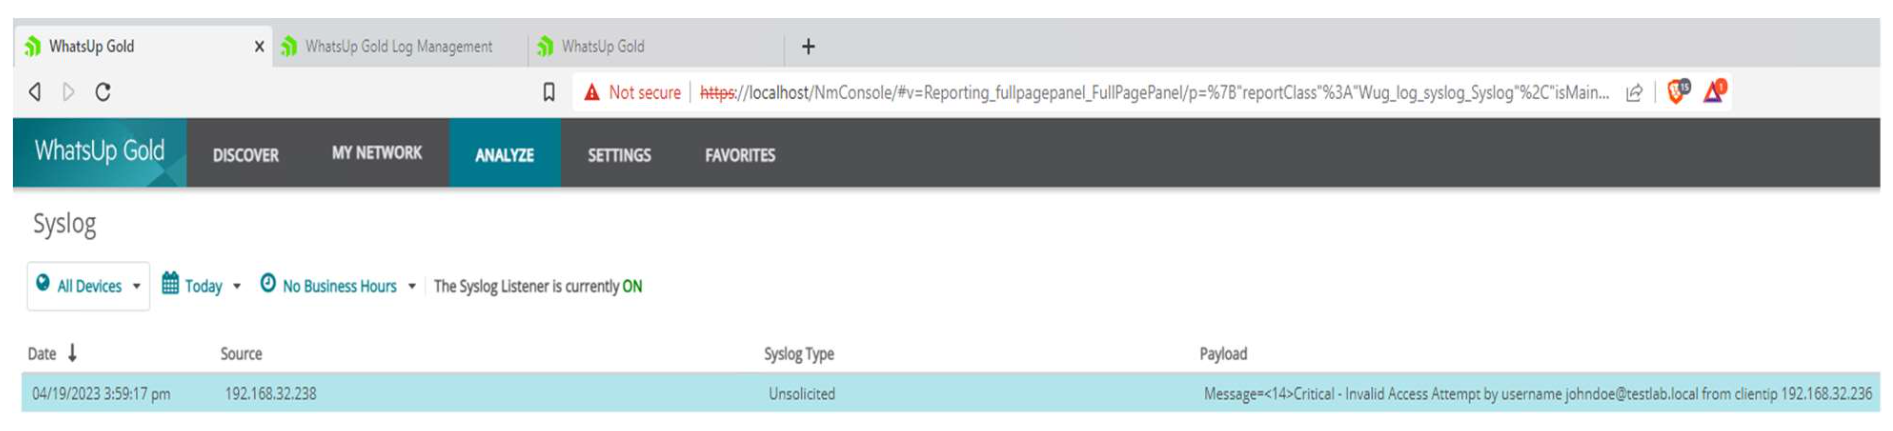
\includegraphics[width=\textwidth]{img/whatsup-gold-alert}}
  \caption{...}\label{fig:whatsup-gold-alert}
\end{figure*}

\begin{enumerate}
\item John Doe enters his office and swipes his access card.
\item The user's group membership is changed from External to
  Internal.  This event is logged to the SIEM service from the
  Raspberry Pi.
\item When the user gets to his desk they access the Web resource
  internally.
\item The DNS points to the LM for DNS resolution of the Web resource
  and since it is an internal request the user is sent to the internal
  service.
\item The ESP requires the user to login.
\item The user's group membership is checked by the ESP SSO system and
  they are connected to the appropriate Web resource.
\item An external threat actor attempts to access the Web resource
  using John Doe's credentials.
\item The DNS points the threat actor to the LM for DNS resolution.
\item Using the correct credentials, the external threat actor logs in
  via the ESP SSO page.
\item The group membership is read as Internal, but the source is
  external, so the threat actor is directed to a ``server
  unavailable'' page and their IP address is logged to the SIEM
  service (see Fig.~\ref{fig:whatsup-gold-alert}).
\end{enumerate}

\subsection{External User with Internal Threat}\label{sec:case-two}

In the second case we are concerned with internal threats: rather than
credentials being leaked externally, they are accessed by a threat
internally, e.g., someone who may have physical access to the user's
desk.  The user, Jane Doe, leaves the office for lunch and swipes her
access card on the RFID reader on the way out.  Her group membership
is set to External.  Meanwhile an internal threat actor attempts to
login from inside the office while the user is away.  They are denied
access and an event is logged to the SIEM service (WUG) as a breach
attempt.  The timeline of events is as follows:

\begin{enumerate}
\item Jane Doe leaves her office and swipes his access card.
\item The user's group membership is changed from Internal to
  External.  This event is logged to the SIEM service from the
  Raspberry Pi.
\item An internal threat actor attempts to access the Web resource
  using Jane Doe's credentials.
\item The DNS points the threat actor to the LM for DNS resolution.
\item Using the correct credentials, the internal threat actor logs in
  via the ESP SSO page.
\item The group membership is read as External, but the source is
  internal, so the threat actor is directed to a ``server
  unavailable'' page.  The event is logged to the SIEM service.
\end{enumerate}
